\documentclass[11pt,letterpaper]{article}

% ---------------------------------------------------------------
%  Motor Moving Side Plate: GD&T scheme and tolerance analysis
%  Compile:  latexmk -pdf main.tex   (pdfLaTeX, TeX Live 2023+ / Overleaf)
% ---------------------------------------------------------------
\usepackage[T1]{fontenc}
\usepackage[sc]{mathpazo}
\usepackage[scaled=0.92]{helvet}
\linespread{1.05}
\usepackage[margin=1in]{geometry}
\usepackage{microtype}
\usepackage{amsmath,amssymb}
\usepackage{graphicx}
\usepackage{booktabs}
\usepackage{threeparttable}
\usepackage{siunitx}
\usepackage{caption}
\usepackage{subcaption}
\usepackage{float}
\usepackage{enumitem}
\usepackage{xcolor}
\usepackage{tikz}
\usetikzlibrary{arrows.meta,decorations.pathreplacing,patterns}
\usepackage{pdflscape}
\usepackage{array}
\usepackage[hidelinks]{hyperref}
\usepackage[capitalise,noabbrev]{cleveref}

\graphicspath{{figures/}}
\sisetup{range-phrase=--, detect-weight=true}
\captionsetup{font=small,labelfont=bf}
\setlist{itemsep=2pt,topsep=4pt}

\definecolor{s1}{HTML}{2A78D6}
\definecolor{s2}{HTML}{EB6834}
\definecolor{s3}{HTML}{1BAF7A}
\definecolor{ink}{HTML}{2B2F33}
\definecolor{muted}{HTML}{8A9196}

% ---------------- GD&T symbols (ASME Y14.5) ----------------
\newcommand{\gsym}[1]{\tikz[baseline=-0.6ex,line width=0.5pt,x=1ex,y=1ex]{#1}}
\newcommand{\Pos}{\gsym{\draw (0,0) circle (0.55); \draw (-0.95,0)--(0.95,0) (0,-0.95)--(0,0.95);}}
\newcommand{\Prof}{\gsym{\draw (-0.9,-0.45)--(0.9,-0.45); \draw (0.8,-0.45) arc (0:180:0.8);}}
\newcommand{\Flat}{\gsym{\draw (-0.95,-0.5)--(0.45,-0.5)--(0.95,0.5)--(-0.45,0.5)--cycle;}}
\newcommand{\Circ}[1]{\tikz[baseline=(c.base)]\node[draw,circle,inner sep=0.4pt,font=\scriptsize\sffamily](c){#1};}
\newcommand{\MMC}{\Circ{M}}
\newcommand{\Proj}{\Circ{P}}
\newcommand{\dia}{$\varnothing$}
\newcommand{\basic}[1]{\fbox{\kern-1pt\small #1\kern-1pt}}
% feature control frame: cells separated by &
\newcommand{\fcf}[1]{{\setlength{\tabcolsep}{3pt}\renewcommand{\arraystretch}{1.1}%
  \begin{tabular}{|*{8}{c|}}\hline #1\\\hline\end{tabular}}}

\title{\textbf{GD\&T Scheme and Tolerance Analysis of an\\Exoskeleton Motor Moving Side Plate}\\[4pt]
\large Datum Selection, Fixed-Fastener Allocation, Projected Zones and a Bracket Coplanarity Stack-Up}
\author{Tien-Hao Chen\\University of California, San Diego}
\date{November 2026}

\begin{document}
\maketitle

\begin{abstract}
\noindent
The Motor Moving Side Plate is a \SI{12.7}{mm} (\SI{0.500}{in}) 6061-T6 plate that couples the
rotor of a CubeMars AKH70-16 actuator to the next link of an upper-limb exoskeleton and carries
two gusset brackets on its side edges. This report documents the ASME Y14.5-2018 drawing
prepared for the part and the calculations behind each tolerance. Datum~A is the face that seats
on the rotor spacer and datum~B is the six-hole bolt pattern that locates the plate on the rotor,
referenced at maximum material condition (MMC). Every position tolerance is derived from the
fixed-fastener relation $T_1+T_2=H-F$. The analysis shows that the plate's own tolerances are
consistent, but it exposes one conflict: the already-machined \dia4.3 bracket holes leave the
bracket only \dia0.1 of position tolerance. Opening them to \dia4.5 resolves it. A
four-contributor stack-up predicts a worst-case offset of \SI{\pm0.50}{mm} (RSS
\SI{\pm0.26}{mm}) between the two faces the bracket must bridge; aligning the parts with a
straightedge before torquing removes the largest term.
\end{abstract}

% =================================================================
\section{Part function and what must be controlled}
\label{sec:function}

The side plate is the first part of the moving link (\cref{fig:drawing}). Its functional
interfaces are:

\begin{enumerate}[label=(\arabic*)]
  \item \textbf{Rotor interface.} The large face seats on a \dia50 rotating spacer and six M4
        screws pass through \dia4.4 clearance holes on a \dia35 pitch circle into the rotor's
        threaded holes. A central \dia7.2 hole clears the rotor hub.
  \item \textbf{Link interface.} Four \dia4.4 holes near the lower edge take M4 screws into the
        end face of the Static Connector, a second \SI{12.7}{mm} plate. The plate's lower edge
        sits flush with the Static Connector's outer face.
  \item \textbf{Bracket interface.} Two M4 threaded holes in each side edge hold an L-shaped
        gusset bracket (\SI{5}{mm} 6061 plate, \dia4.3 holes) whose other leg is bolted to the
        Static Connector. The companion FEA report shows that these brackets carry most of the
        joint torque, so they only work if they seat flat on both parts.
\end{enumerate}

The tolerancing question is therefore: \emph{how far can each feature move and still let every
screw assemble and the bracket seat flat?} Sizes, locations and the outer profile are all set
from that question rather than from generic title-block tolerances.

% =================================================================
\section{Datum reference frame}
\label{sec:datums}

\paragraph{Datum A: the spacer-contact face.}
This face is the primary datum because it is the surface the part physically seats on in
assembly; it removes three degrees of freedom (one translation, two rotations). It carries a
flatness tolerance of \fcf{\Flat & 0.1} so that the six screws clamp the plate without rocking.
The plate is bought as \SI{0.500}{in} stock and is not faced, so its thickness is dimensioned
as \texttt{12.7 (0.500 STOCK)} rather than as a machined size.

\paragraph{Datum B: the 6\texttimes\dia4.4 pattern at MMC.}
The secondary datum is the bolt pattern, not an outer edge, because the screws, not the edges,
locate the part on the rotor. Choosing the edges would make inspection measure the part
differently from the way it functions. The pattern is controlled as
\fcf{\Pos & \dia0.2\,\MMC & A} and labelled datum~B. Because B is a feature of size, it is
referenced at MMC (\textsf{B}\MMC) in every downstream frame. The datum feature simulator is then
a set of six fixed pins at the pattern's virtual condition,
\begin{equation}
  \mathrm{VC} = \text{MMC hole} - \text{position tolerance} = 4.40 - 0.20 = \SI{4.20}{mm},
\end{equation}
and any clearance between the actual holes and those pins is \emph{datum shift}: extra freedom
the inspector may use, exactly as the real screws allow the part to shift on the rotor.
B removes the remaining two translations and the rotation about A, so no tertiary datum is
needed.

% =================================================================
\section{Drawing summary}
\label{sec:summary}

\Cref{tab:fcf} lists every geometric control on the drawing. All locating dimensions for these
features are basic (boxed); the title-block tolerances (one place $\pm0.2$, two places
$\pm0.1$, angles $\pm0.5^\circ$) apply only to the remaining non-basic dimensions.

\begin{table}[H]
\centering
\small
\caption{Geometric controls on the Moving Side Plate drawing.}
\label{tab:fcf}
\renewcommand{\arraystretch}{1.25}
\begin{tabular}{@{}p{3.2cm}p{4.3cm}p{6.6cm}@{}}
\toprule
Feature & Control & Purpose \\
\midrule
Spacer face (A) & \fcf{\Flat & 0.1} & Seats without rocking under six-screw clamp \\
6\texttimes\dia4.4$^{+0.15}_{\;\;0}$ (B) & \fcf{\Pos & \dia0.2\,\MMC & A} & Assembles to rotor M4 holes; defines datum B \\
\dia7.2$^{+0.3}_{\;\;0}$ & \fcf{\Pos & \dia0.5 & A & B\MMC} & Hub clearance only; loose tolerance \\
4\texttimes\dia4.4$^{+0.15}_{\;\;0}$ & \fcf{\Pos & \dia0.2\,\MMC & A & B\MMC} & Assembles to Static Connector M4 holes \\
4\texttimes M4\texttimes0.7-6H, 2 per side & \fcf{\Pos & \dia0.2\,\Proj\,5 & A & B\MMC} & Bracket screws; zone projected through \SI{5}{mm} bracket \\
Outer profile, all around & \fcf{\Prof & 0.2 & A & B\MMC} & Side edges and lower edge seat the bracket and align with the Static Connector \\
\bottomrule
\end{tabular}
\end{table}

\paragraph{Why profile instead of size tolerances on the outline.}
The outline is waterjet cut. A single all-around profile tolerance controls the location,
orientation and form of the side edges, lower edge and \basic{R35} arc relative to the datum
frame in one frame, which a set of $\pm$ dimensions cannot do: under Rule~\#1, a $\pm$ width
says nothing about where the edges sit relative to the bolt pattern. A zone of 0.2 (\SI{\pm0.1}{mm})
is near the edge of typical waterjet capability (\SIrange{\pm0.1}{\pm0.15}{mm}), which is why
note~4 on the drawing requires the cut taper to stay inside the zone.

\paragraph{Symmetry.}
The 4\texttimes\dia4.4 pattern (\basic{18}, \basic{45}) and the \basic{70} width are dimensioned
symmetrically about a vertical centerline drawn through the datum~B pattern centre, which ties
their horizontal location to datum~B.

% =================================================================
\section{Fixed-fastener tolerance allocation}
\label{sec:fastener}

\subsection{Relation}

Every bolted interface on this part is a \emph{fixed-fastener} case: the screw is threaded into
one part (and therefore cannot move relative to it) and passes through a clearance hole in the
other. For the screw to assemble when both parts are at MMC and their position errors are at
the limit in opposite directions,
\begin{equation}
  T_1 + T_2 = H - F,
  \label{eq:fixed}
\end{equation}
where $H$ is the MMC (smallest) clearance-hole diameter, $F$ is the MMC (largest) fastener
diameter (\SI{4.0}{mm} for M4), and $T_1$, $T_2$ are the diametral position tolerances of the
clearance hole and the threaded hole. For comparison, the floating-fastener case (clearance holes
in both parts, nut on the end) allows $T = H - F$ for \emph{each} part. Fixed fasteners must
share the budget, which is why they are the stricter case.

\subsection{Allocation}

\begin{table}[H]
\centering
\small
\caption{Fixed-fastener allocation for each M4 joint. All values in mm, diametral.}
\label{tab:alloc}
\begin{threeparttable}
\begin{tabular}{@{}lccccc@{}}
\toprule
Joint & $H$ & $F$ & $H-F$ & Side plate & Mating part \\
\midrule
6\texttimes\ side plate $\rightarrow$ rotor threads        & 4.4 & 4.0 & 0.4 & \dia0.2\,\MMC & \dia0.2\tnote{a} \\
4\texttimes\ side plate $\rightarrow$ Static Connector     & 4.4 & 4.0 & 0.4 & \dia0.2\,\MMC & \dia0.2\,\Proj\tnote{b} \\
Bracket (\dia4.3) $\rightarrow$ side-plate threads          & 4.3 & 4.0 & 0.3 & \dia0.2\,\Proj\,5 & \textcolor{s2}{\textbf{\dia0.1}} \\
Bracket, reworked to \dia4.5                                & 4.5 & 4.0 & 0.5 & \dia0.2\,\Proj\,5 & \dia0.3\,\MMC \\
\bottomrule
\end{tabular}
\begin{tablenotes}\footnotesize
  \item[a] Actuator vendor tolerance, not published; assumed. Its projected height is the
           side plate plus spacer, $12.7 + 15 = \SI{27.7}{mm}$.
  \item[b] To be specified on the Static Connector drawing, projected \SI{12.7}{mm}.
\end{tablenotes}
\end{threeparttable}
\end{table}

The two \dia4.4 patterns split the \SI{0.4}{mm} budget evenly. The bracket joint, however, has
only \SI{0.3}{mm} because the bracket holes were already machined at \dia4.3 (a close-fit M4
clearance). With \dia0.2 assigned to the side-plate threads, the bracket is left with \dia0.1,
which is not realistic for a hand-drilled or waterjet hole. Two fixes were considered:

\begin{itemize}
  \item \textbf{Split 0.15 / 0.15.} Keeps the existing bracket, but tightens the side-plate
        threads, which are drilled into a \SI{12.7}{mm} edge after the profile cut and are the
        hardest features on the part to hold.
  \item \textbf{Open the bracket holes to \dia4.5 (adopted).} Enlarging an existing hole with a
        drill is a few minutes of rework, raises the budget to \SI{0.5}{mm}, and gives the
        bracket \dia0.3 at MMC while leaving the side plate unchanged.
\end{itemize}

\subsection{Bonus tolerance}

Because the clearance holes are toleranced at MMC, the allowed position error grows as the
hole departs from MMC, while the virtual condition (\SI{4.20}{mm}) stays fixed (\cref{tab:bonus}).
A functional gauge with \dia4.20 pins therefore accepts exactly the parts that assemble.

\begin{table}[H]
\centering
\small
\caption{Bonus tolerance for the \dia4.4$^{+0.15}_{\;\;0}$ holes.}
\label{tab:bonus}
\begin{tabular}{@{}cccc@{}}
\toprule
Actual hole size & Bonus & Allowed position & Virtual condition \\
\midrule
4.40 (MMC) & 0.00 & \dia0.20 & 4.20 \\
4.45       & 0.05 & \dia0.25 & 4.20 \\
4.50       & 0.10 & \dia0.30 & 4.20 \\
4.55 (LMC) & 0.15 & \dia0.35 & 4.20 \\
\bottomrule
\end{tabular}
\end{table}

% =================================================================
\section{Projected tolerance zone for the bracket threads}
\label{sec:projected}

A position tolerance on a threaded hole normally applies over the depth of the thread. The
screw, however, has to pass through the bracket \emph{above} the hole, and a tilted thread axis
keeps diverging outside the part (\cref{fig:proj}).

With a \dia0.2 zone over the \SI{8}{mm} full-thread depth, the worst tilt runs from one side of
the zone at the bottom of the thread to the other side at the surface, a slope of
$0.2/8 = 0.025$. At height $h$ above the surface the axis is offset from true position by
\begin{equation}
  e(h) = 0.1 + 0.025\,h \quad\Rightarrow\quad e(5) = \SI{0.225}{mm},
\end{equation}
which corresponds to a \dia0.45 zone at the top of the bracket, more than double the value the
allocation in \cref{tab:alloc} assumed. Specifying \fcf{\Pos & \dia0.2\,\Proj\,5 & A & B\MMC}
moves the \dia0.2 zone to the \SI{5}{mm} the bracket actually occupies, so the allocation holds
through the full mating thickness. It is inspected with a threaded gauge pin that protrudes
\SI{5}{mm}.

\begin{figure}[H]
\centering
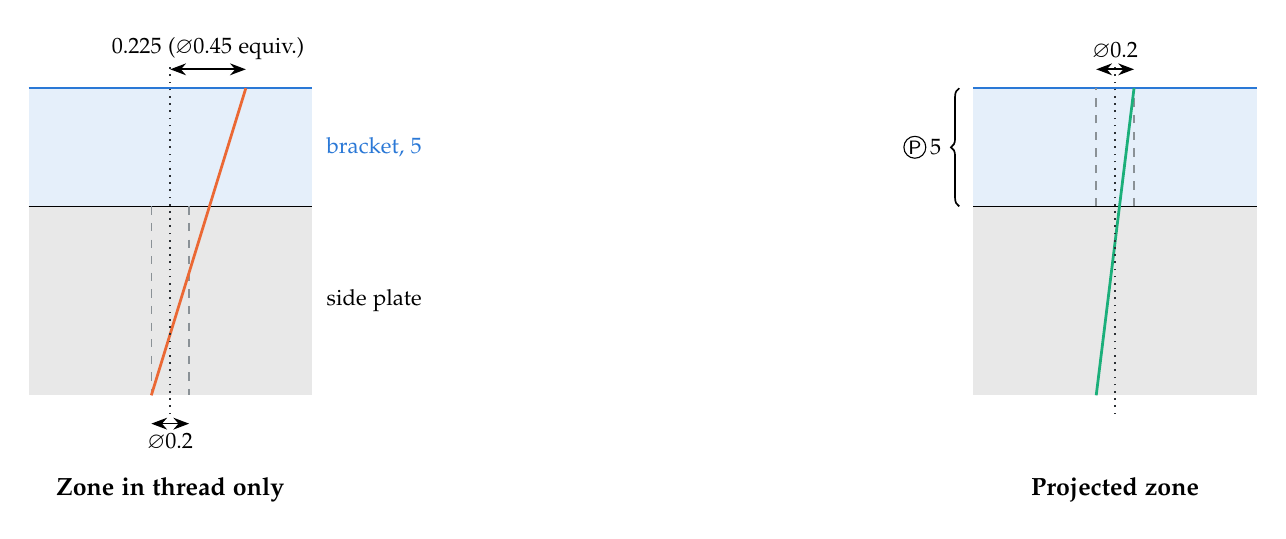
\begin{tikzpicture}[x=6mm,y=6mm,line width=0.6pt,>=Stealth]
  % ---- left: without projection
  \begin{scope}
    \fill[gray!18] (-3,0) rectangle (3,-4);
    \draw (-3,0)--(3,0);
    \node[font=\footnotesize,anchor=west] at (3.1,-2) {side plate};
    \fill[s1!12] (-3,0) rectangle (3,2.5);
    \draw[s1] (-3,2.5)--(3,2.5);
    \node[font=\footnotesize,anchor=west,s1] at (3.1,1.25) {bracket, 5};
    % zone in part
    \draw[dashed,muted] (-0.4,0)--(-0.4,-4) (0.4,0)--(0.4,-4);
    % tilted axis
    \draw[s2,line width=1pt] (-0.4,-4)--(1.6,2.5);
    \draw[ink,dotted] (0,-4.4)--(0,3.0);
    \draw[<->,font=\footnotesize] (-0.4,-4.6)--(0.4,-4.6) node[midway,below] {\dia0.2};
    \draw[<->,font=\footnotesize] (0,2.9)--(1.6,2.9) node[midway,above] {0.225 (\dia0.45 equiv.)};
    \node[font=\small\bfseries] at (0,-6) {Zone in thread only};
  \end{scope}
  % ---- right: projected
  \begin{scope}[xshift=12cm]
    \fill[gray!18] (-3,0) rectangle (3,-4);
    \draw (-3,0)--(3,0);
    \fill[s1!12] (-3,0) rectangle (3,2.5);
    \draw[s1] (-3,2.5)--(3,2.5);
    \draw[dashed,muted] (-0.4,0)--(-0.4,2.5) (0.4,0)--(0.4,2.5);
    \draw[s3,line width=1pt] (-0.4,-4)--(0.4,2.5);
    \draw[ink,dotted] (0,-4.4)--(0,3.0);
    \draw[<->,font=\footnotesize] (-0.4,2.9)--(0.4,2.9) node[midway,above] {\dia0.2};
    \draw[decorate,decoration={brace,amplitude=3pt}] (-3.3,0)--(-3.3,2.5)
      node[midway,left=3pt,font=\footnotesize] {\Proj\,5};
    \node[font=\small\bfseries] at (0,-6) {Projected zone};
  \end{scope}
\end{tikzpicture}
\caption{Worst-case thread axis. Left: a \dia0.2 zone applied inside the \SI{8}{mm} thread lets
the screw axis drift to \SI{0.225}{mm} from true position at the top of the bracket. Right: the
projected zone holds \dia0.2 through the bracket thickness.}
\label{fig:proj}
\end{figure}

% =================================================================
\section{Bracket coplanarity stack-up}
\label{sec:stack}

\subsection{Requirement}

Each bracket is a flat plate bolted to two different parts: the side edge of this plate and the
side face of the Static Connector. If those two faces are not coplanar, the bracket touches one
part first and the screws must bend it into contact. That adds stress the FEA did not include
and reduces the stiffness the brackets contribute; the FEA model assumed the faces were
perfectly flush. The quantity of interest is therefore the offset $g$, normal to the bracket,
between the side-plate edge and the Static Connector face.

\subsection{Contributors}

The two parts are located relative to each other only by the 4\texttimes M4 screws through the
lower \dia4.4 holes, so the chain is: side-plate edge $\rightarrow$ side-plate holes
$\rightarrow$ screws $\rightarrow$ Static Connector threads $\rightarrow$ Static Connector face.

\begin{table}[H]
\centering
\small
\caption{One-dimensional stack-up of the offset $g$ (mm), holes at MMC.}
\label{tab:stack}
\begin{threeparttable}
\begin{tabular}{@{}clcc@{}}
\toprule
\# & Contributor & Source & $\pm$ \\
\midrule
1 & Radial clearance of M4 in \dia4.4 hole & $(4.4-4.0)/2$ & 0.20 \\
2 & Side-plate 4\texttimes\ hole position & \dia0.2 / 2 & 0.10 \\
3 & Static Connector thread position\tnote{a} & \dia0.2 / 2 & 0.10 \\
4 & Side-plate edge profile & 0.2 / 2 & 0.10 \\
\midrule
  & Worst case $\sum t_i$ & & \textbf{0.50} \\
  & RSS $\sqrt{\sum t_i^2}$ & & \textbf{0.26} \\
\bottomrule
\end{tabular}
\begin{tablenotes}\footnotesize
  \item[a] Assumes the Static Connector side face is its datum, so its threads are located
           directly from it and the face contributes no separate term.
\end{tablenotes}
\end{threeparttable}
\end{table}

\noindent
Two remarks qualify these numbers. First, the clearance term is not random in the statistical
sense: it is set by how the assembler pushes the parts before tightening, so in practice it
behaves more like a bias than a normal variable, and the RSS value is optimistic unless
assembly is controlled. Second, with the holes at LMC the extra clearance and the bonus
tolerance each add \SI{0.075}{mm}, raising the worst case to \SI{\pm0.65}{mm}.

\subsection{Mitigation}

The clearance term is the largest, and it is also the only one that can be removed at
assembly without changing any drawing:

\begin{itemize}
  \item \textbf{Straightedge alignment (adopted for the prototype).} Clamp a precision
        straightedge across the side-plate edge and the Static Connector face, then torque the
        four M4 screws. This eliminates term~1: worst case $\pm0.30$, RSS
        $\sqrt{3}\times0.1 = \pm0.17$. Cost: none.
  \item \textbf{Dowel pins.} Two reamed \dia3 dowels between the parts replace the screw
        clearance with a press or slip fit, making the alignment repeatable after disassembly.
        Worth adopting if the joint is serviced often.
  \item \textbf{Shim or face after assembly.} Shim the bracket on the low side, or skim both
        faces flush in one setup. Effective but adds a process step.
\end{itemize}

Slotting the bracket holes would ease in-plane misalignment between the four bracket screws,
but it does not reduce $g$, which is normal to the bracket.

% =================================================================
\section{Inspection plan}
\label{sec:inspection}

\begin{itemize}
  \item \textbf{Datum A flatness:} surface plate and dial indicator, or CMM, \SI{0.1}{mm}.
  \item \textbf{6\texttimes\ and 4\texttimes\ \dia4.4 holes:} hole size with pin gauges
        (4.40 go / 4.55 no-go); position with a functional gauge: six \dia4.20 pins (datum B)
        plus four \dia4.20 pins at the basic locations, with the part resting on a flat
        datum~A plate. A part that drops onto all ten pins is acceptable.
  \item \textbf{Side threads:} M4-6H go/no-go plug gauge; position with threaded gauge pins
        protruding \SI{5}{mm}, measured on a CMM against the datum A/B frame.
  \item \textbf{Outer profile:} CMM scan of the side edges, lower edge and R35 arc, best-fit
        to the datum frame allowing the B\MMC\ shift; every point within \SI{\pm0.1}{mm}.
\end{itemize}

% =================================================================
\section{Conclusions}
\label{sec:conclusion}

\begin{enumerate}
  \item The datum frame follows function: A is the seating face, B is the bolt pattern that
        locates the plate on the rotor, referenced at MMC so inspection permits the same shift
        the screws permit.
  \item All position tolerances follow from $T_1+T_2=H-F$. The two \dia4.4 patterns split a
        \SI{0.4}{mm} budget evenly at \dia0.2\MMC.
  \item The existing \dia4.3 bracket holes leave the bracket only \dia0.1; opening them to
        \dia4.5 gives \dia0.3 with a few minutes of rework.
  \item A projected zone of \SI{5}{mm} on the side threads is required: without it the screw
        axis can drift to the equivalent of \dia0.45 at the top of the bracket.
  \item The bracket faces can be offset by up to \SI{\pm0.50}{mm} (RSS \SI{\pm0.26}{mm}).
        Straightedge alignment before torquing removes the dominant clearance term and reduces
        this to \SI{\pm0.30}{mm} (RSS \SI{\pm0.17}{mm}).
\end{enumerate}

% =================================================================
\begin{landscape}
\begin{figure}[p]
\centering
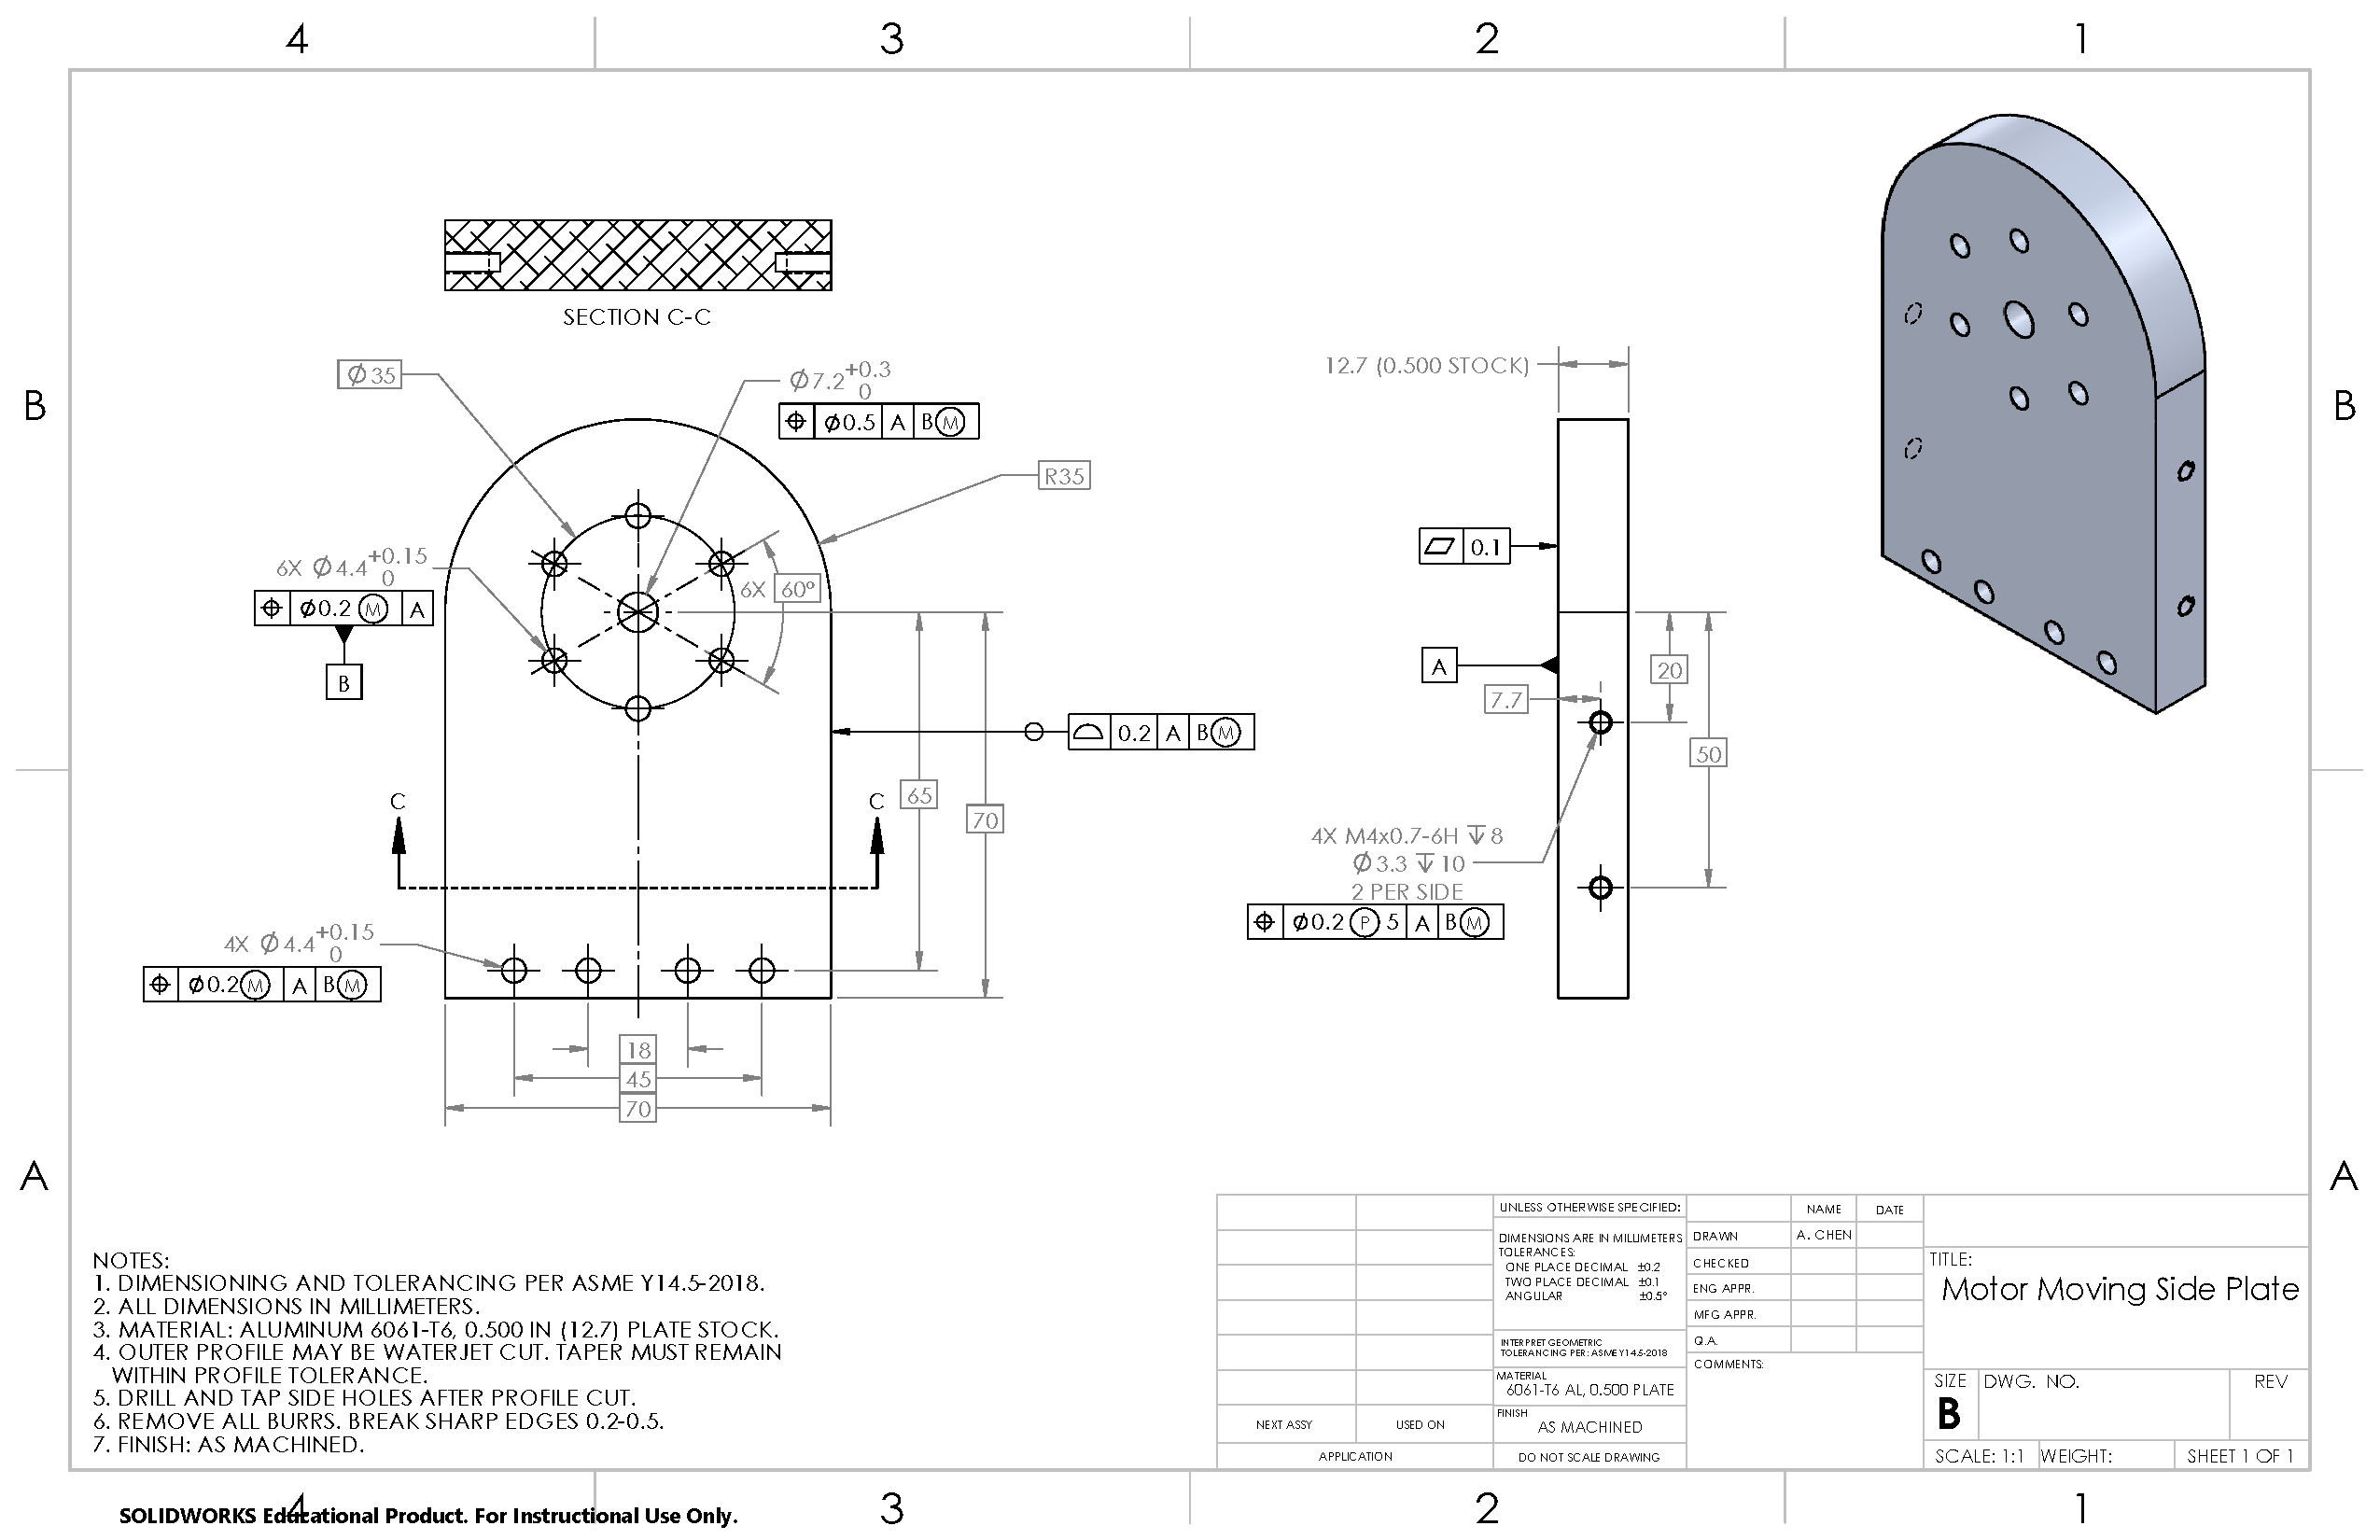
\includegraphics[width=\linewidth,height=0.86\textheight,keepaspectratio]{MSP_drawing.pdf}
\caption{ASME Y14.5-2018 drawing of the Motor Moving Side Plate (B size, scaled to fit).}
\label{fig:drawing}
\end{figure}
\end{landscape}

\end{document}
